\begin{frame}
    \centering
    \Huge{Sistemas Operativos para Móviles}
\end{frame}

\frame{
\frametitle{PCs vs móviles}
\begin{figure}[htb]
\centering
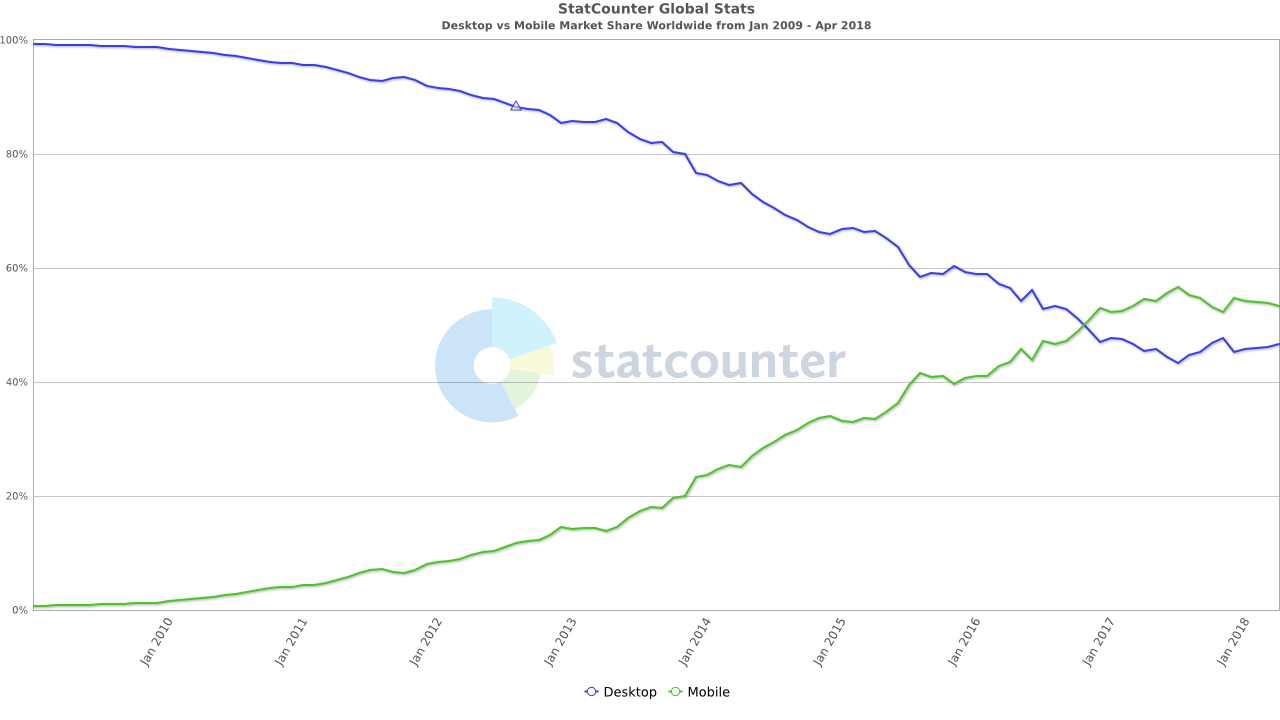
\includegraphics[width=0.8\textwidth]{images/platform.png}
\caption{Comparativa de uso de las plataformas}
\label{fig:Comparativa de uso de las plataformas}
\end{figure}
}
\frame{
\frametitle{Distribución de S.O. (móviles)}
\begin{figure}[htb]
\centering
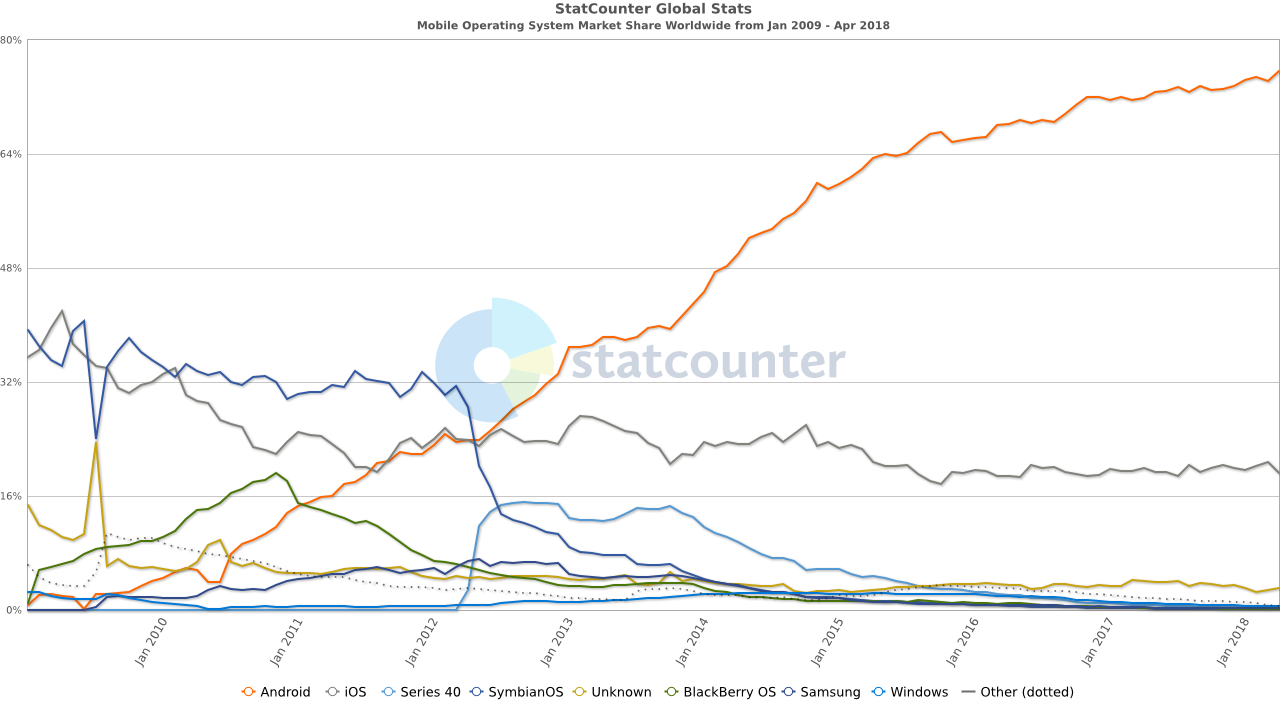
\includegraphics[width=0.8\textwidth]{images/so.png}
\caption{Comparativa de uso de S.O.}
\label{fig:Comparativa de uso de S.O.}
\end{figure}
}

\frame{
\frametitle{Android}
\begin{block}{Historia:}
\begin{itemize}
\item 2003: Andy Rubin funda Android Inc
\item 2005: Google compra Android Inc
\item 2008: Se presenta la primera versión de Android (1.0 Apple Pie)
\end{itemize}
\end{block}
\begin{itemize}
\item Apps: Android SDK, Java
\item Play Store, Aptoide, F-Droid...
\item Altamente personalizable (apps de terceros)
\item Una actualización "grande" al año
\item Última versión: 8.1 Oreo
\end{itemize}
}

\frame{
\frametitle{iOS}
\begin{block}{Historia:}
\begin{itemize}
\item 2007: Se anuncia iPhone OS con el primer iPhone
\item 2008: App Store y SDK
\item 2010: Se cambia el nombre a iOS
\end{itemize}
\end{block}
\begin{itemize}
\item Apps: iPhone SDK, Swift, Objective-C
\item App Store
\item SDK sólo para Mac
\item Muy poco personalizable
\item Una actualización "grande" al año
\item Última versión: 11
\end{itemize}
}

\frame {
\frametitle{Windows 10 Mobile}
\begin{itemize}
\item Versión de Windows 10 para móviles
\item Aplicaciones unificadas (PCs, móviles, tablets)
\item Retrocompatibilidad con apps de Windows Phone 8 i 8.1
\item Tienda de aplicaciones de Microsoft
\item Conversión a interfaz de escritorio
\end{itemize}
}

\frame{
\frametitle{Ubuntu Touch}
\begin{block}{Historia:}
\begin{itemize}
\item 2011: Se anuncia el proyecto
\item 2015: Primer dispsitivo con Ubuntu Touch (BQ)
\item 2016: Cannonical abandona el proyecto
\end{itemize}
\end{block}
\begin{itemize}
\item Versión de Ubuntu para móviles
\item Mantenido por UBports (anteriormente por Cannonical)
\item Apps: JS, Qt, C++, Python, Go, QML, HTML5
\item OpenStore
\item Compatibilidad con aplicaciones de escritorio y Android (algunos dispositivos)
\end{itemize}
}

\frame{
\frametitle{Plasma Mobile}
\begin{itemize}
\item Sistema operativo de KDE
\item Basado en Kubuntu (se puede integrar con otras distribuciones Linux)
\item Se puden desarrollar apps nativas o portarlas (Ubuntu Touch)
\end{itemize}
}

\frame{
\frametitle{Android vs iOS vs Windows}
\begin{figure}[htb]
\centering
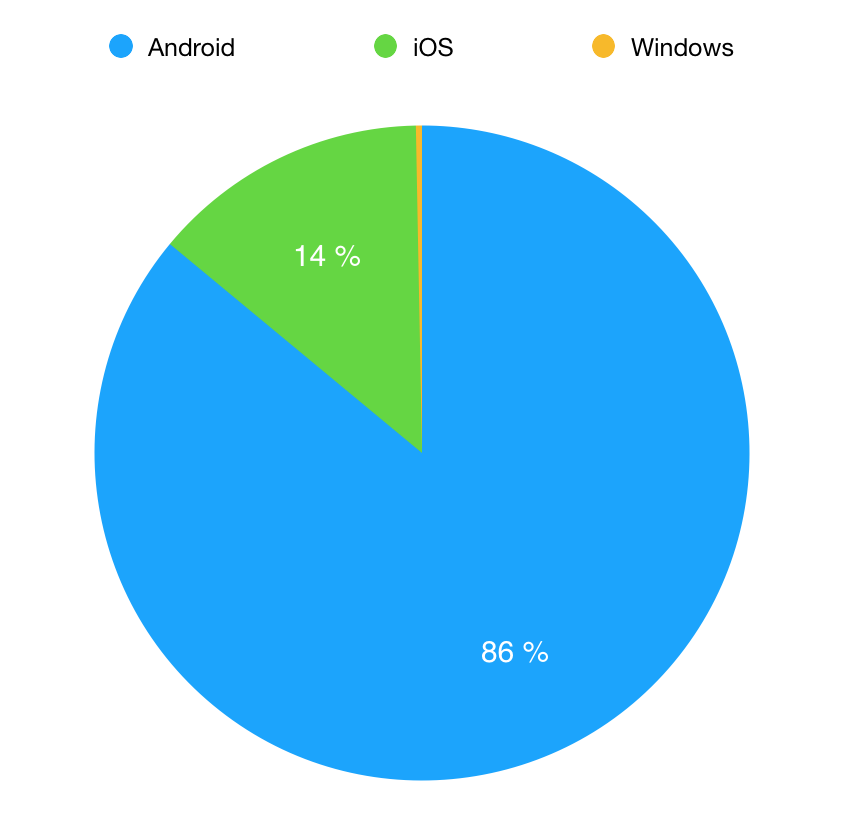
\includegraphics[height=0.8\textheight]{images/grafico_SO.png}
\caption{Android vs iOS vs Windows}
\label{fig:Android vs iOS vs Windows}
\end{figure}
}
